\documentclass[border=2pt]{standalone}
\usepackage{amsmath}
\usepackage{tikz}
\usetikzlibrary{intersections}
\usetikzlibrary{arrows}
\usetikzlibrary{quotes,angles}
\usepackage{amsmath}
\usepackage{xcolor}

\begin{document}

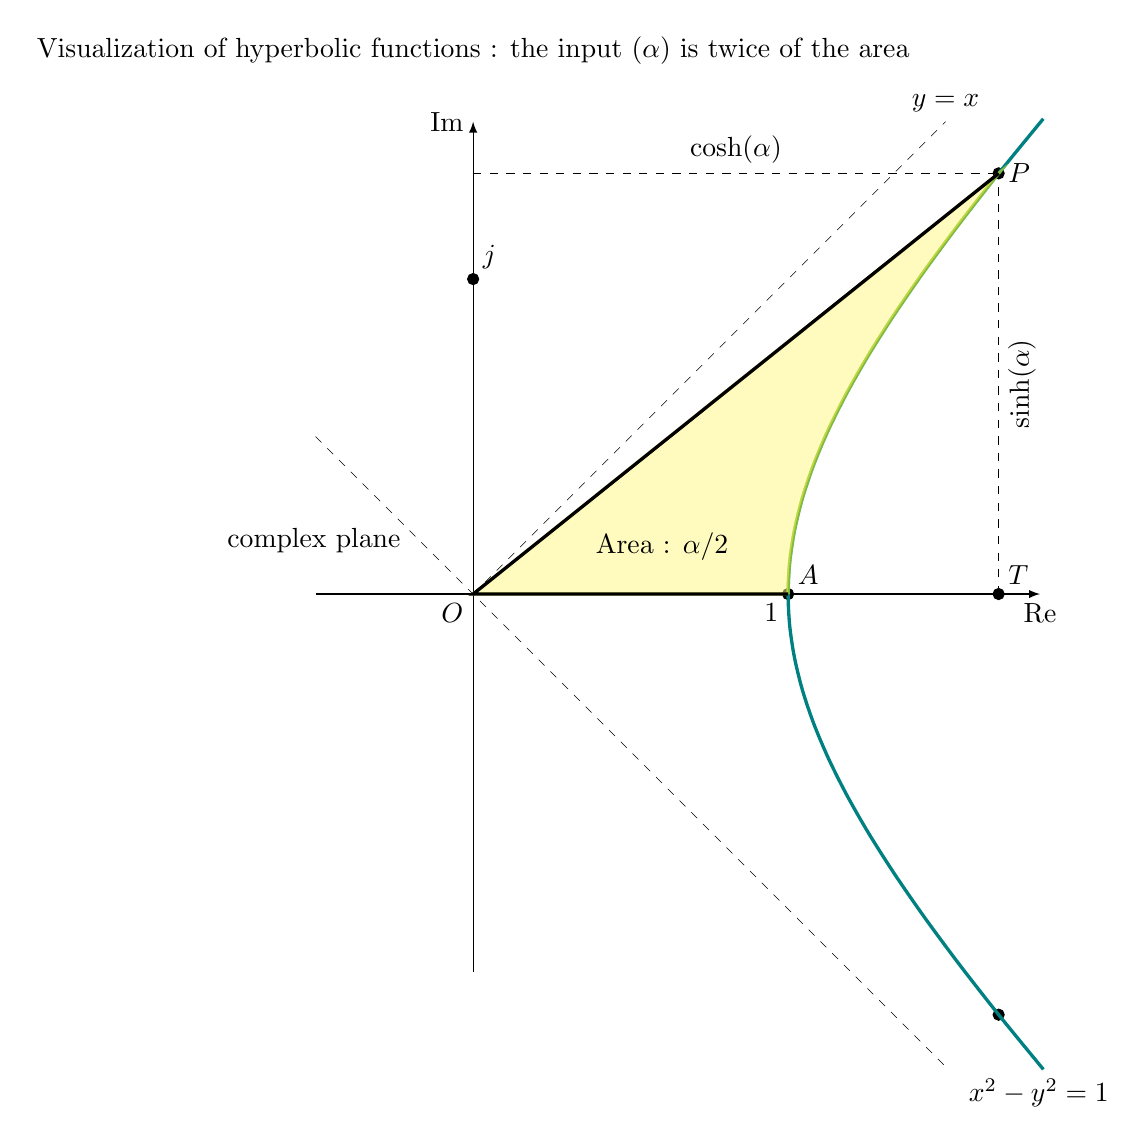
\begin{tikzpicture}[scale=4]

% Draw x and y axis lines
\draw [->,>=latex] (-0.5,0) -- (1.80,0) node [below] {$\mathrm{Re}$};
\draw [->,>=latex] (0,-1.2) -- (0,1.50) node [left ] {$\mathrm{Im}$};
\node[above left] at (-0.2, 0.1) {complex plane} ;
\node[below left] at ( 0.0, 0.0) {$O$} ;
\filldraw[black] (1,0) circle (0.5pt) node[below left ] {$1$} node[above right] {$A$} ;
\filldraw[black] (0,1) circle (0.5pt) node[above right] {$j$} ;
\node[above] at (0.0,1.65) {Visualization of hyperbolic functions : the input $(\alpha)$ is twice of the area};

% Draw a circle at the origin of radius 1
%\draw (0,0) circle (1);

\draw [very thin, dashed] (-0.0,-0.0) -- ( 1.5, 1.5) node[above] {$y=x$} ;
\draw [very thin, dashed] (-0.5, 0.5) -- ( 1.5,-1.5) ;

\pgfmathsetmacro{\angle}{1.1}
\pgfmathsetmacro{\length}{\angle}

\filldraw[black] ({ cosh(\angle)}, { sinh(\angle)}) circle (0.5pt) node[right] {$P$} ;
\filldraw[black] ({ cosh(\angle)}, {-sinh(\angle)}) circle (0.5pt) ;
\filldraw[black] ({ cosh(\angle)}, 0) circle (0.5pt) node[above right] {$T$} ;

\draw [very thin, dashed] ( 0.0, { sinh(\angle)}) -- node[above] {$\cosh(\alpha)$}  ({ cosh(\angle)}, { sinh(\angle)}) ;
\draw [very thin, dashed] ( { cosh(\angle)}, 0.0) -- node[below, rotate=90] {$\sinh(\alpha)$}  ({ cosh(\angle)}, { sinh(\angle)}) ;

% 画双曲线
\draw[very thick,smooth,variable=\x, color=teal] plot[domain=-\angle-0.1:\angle+0.1] ({ cosh(\x)}, {sinh(\x)}) ;
\node[below right] at ({ cosh(\angle-0.1)}, {-sinh(\angle+0.1)}) {$x^2 - y^2 = 1$} ;
%\draw[very thick,smooth,variable=\x, color=teal] plot[domain=-1.2:1.2] ({-cosh(\x)}, {sinh(\x)}) ;

\filldraw[very thick, draw=yellow,fill=yellow!50,opacity=0.5]
[smooth,variable=\x] plot[domain=-0:\angle] ({ cosh(\x)}, {sinh(\x)})
 -- ({ cosh(\angle)}, { sinh(\angle)}) -- (0,0) -- (1,0)
;
\draw[very thick] ({ cosh(\angle)}, { sinh(\angle)}) -- (0,0) -- (1,0) ;

% Draw a string at center.
\node at (0.6, 0.15) {Area : $\alpha/2$};





\end{tikzpicture}

\end{document}
